
\chapter{Background Mathematics}
\label{sec:background}

\epigraph{Try as you may you just can't get away from Mathematics }{\textit{That's Mathematics by Tom Lehrer}}

\section{Background and References}
As this is a maths module there is a lot of assumed background.  This means that to understand the material in the module and to be able to solve the tutorial problems, you need to have a experience with a variety of mathematical techniques such as:
\begin{itemize}
%\setlength{\itemsep}{-5pt}
    \item solving linear equation,
    \item solving quadratic equations
    \item using trigonometry,
    \item knowning some simple functions.
\end{itemize}

These topics will be familiar to many of you. However, it may have been a while since some of you studied mathematics and I am aiming to briefly introduce any new mathematical topics when we need them. However, I also want to link to some extra resources where you can brush up on your maths beforehand.\\


A great resource is the website \href{https://tutorial.math.lamar.edu/}{Pauls Online Math Notes}. The website contains notes for a variety of mathematics courses including algebra and calculus. The most useful background materials are the Algebra and trigonometry review \href{https://tutorial.math.lamar.edu/Extras/AlgebraTrigReview/AlgebraTrigIntro.aspx}{linked here} and the preliminaries section of the algebra notes, \href{https://tutorial.math.lamar.edu/Classes/Alg/Preliminaries.aspx}{linked here}.\\

As the module goes on I may add more background resources or add some examples.\\

%The essential maths skills needed for studying physics at this level are nicely summarised in \citep{garrett2015essential}. It is worth having a look at this book if you want to revise the maths background.

\section{Polynomials and roots}
One of the most common examples of a function that we will meet is a polynomial. These are functions wher ethe variable $x$ is sent to a sum of powers of $x$,
\begin{equation}
p(x)=a_{n}x^{n}+a_{n-1}x^{n-1}\cdots +a_{1}x+a_{0}.
\label{eq: polynomial}
\end{equation}
If we plot a polynomial, e.g. produce the graph $(x,y=p(x))$, then the locations where the plot cuts the $x$-axis, where $y=p(x)=0$, are called the zeros or roots. For a linear equation we solve it via rearrangement, see \cref{sec: rearranging}. For a quadratic equation like
\begin{equation*}
ax^{2}+bx+c=0,
\end{equation*}
we solve it using the quadratic formula
\begin{equation}
x=\frac{-b\pm\sqrt{b^{2}-4ac}}{2a}.
\end{equation}

As an example consider the quadratic equation
\begin{equation*}
2x^{2}-4x-2=0.
\end{equation*}
To apply the quadratic formula we compare this specific equation to the general quadratic equation above, and note that $a=2,b=-4,c=-2$. The quadratic formula thus gives
\begin{align*}
x 	&=\frac{4\pm\sqrt{4^{2}+4\times2\times2}}{4}\\
	&=\frac{4\pm\sqrt{16+16}}{4}\\
	&=1\pm\frac{\sqrt{32}}{4}\\
	&=1\pm\frac{\sqrt{16}\sqrt{2}}{4}\\
	&=1\pm\sqrt{2}.
\end{align*}
So the two roots are $1+\sqrt{2}$, $1-\sqrt{2}$.\\

Note that we can guess the roots by looking at the polynomial. A quadratic can always be written as 
\begin{align*}
a(x-\alpha)(x-\beta)	&=a\left(x^{2}-(\alpha+\beta)x+\alpha\beta\right)\\
				&=ax^{2}-a\left(\alpha+\beta\right)+a\alpha\beta.
\end{align*}
So the product of the roots is related to the constant term, and the sum of the roots is related to the linear term. This means that we can guess one of the roots by looking at the factors of the constant term. For quadratics we do not need to do this, but with higher order equations this is very useful.\\

For higher order polynomials we do not have a formula to find the solutions\footnote{The exception is cubic equations. There is a cubic formula. However, it is fairly complicated and there is no point in trying to use it.} In this case we use the higher order versions of the above identity that the constant term in the polynomial is related to the product of the roots. We can then use a technique like polynomial long division to reduce the order of the equation.\\

Consider the equation
\begin{equation*}
x^{3}+x^{2}-x-1=0
\end{equation*}
Since $(x-a)(x-b)(x-c)$ has a constant term $-abc$ we see that the product of the three roots is $1$. This means that we can guess that $1$ is one of the roots. 

\begin{warpprint}
We can the perform polynomial long division to find that
\begin{equation*}
\polylongdiv{x^3+x^2-x-1}{x-1}
\end{equation*}
This means that we can rewrite
\begin{equation*}
x^{3}+x^{2}-x-1=(x-1)(x^{2}+2x+1),
\end{equation*}
and then we can either factorise the quadratic directly or use the quadratic formula. Note that we could also solve this case using polynomial long division by noting that the product of the roots is $1$ so we can guess that $-1$ is a repeated root and calculate
\begin{equation*}
\polylongdiv{x^{2}+2x+1}{x+1}
\end{equation*}
\end{warpprint}

\begin{warpHTML}
We then need to use polynomial long division to factor out this root and reduce our equation to a quadratic that we can then solve. If you read the pdf version of these notes then it is nice and easy to include examples of polynomial long division. Unfortunately in the HTML version this does not display properly so we need to proceed more slowly.\\

You may remember for your time at school learning about long division, the idea is you want to know how many times a small number goes into a big number. You are likely familiar with a couple of notations for this such as $a\div b$ or $a/b$.  When the number we are dividing, $a$ involves lots of digits it is easier to write it as
\begin{equation*}
b)\overline{a}.
\end{equation*}
Long division is the process of carrying out these calculations.\\

Consider the problem of dividing $1260257$ by 37, this is done as follows
\begin{align*}
& \phantom{++}34061\\
37&)\overline{1260257}\\
&\underline{1110000}
&\phantom{1}150257
&\phantom{1}\underline{148000}
&\phantom{111}2257
&\phantom{111}\underline{2220}\\
&\phantom{11111}37
\end{align*}
For understanding the steps I recommend having a look at the Wikipedia article on long division if you want a refresher as it contains lots of examples. The key idea is that you work term by term, typically ignoring the digits on the right, until you have a number that is bigger than your starting one, in this case $37$. Then you write down how many times 37 goes it to that number, in this case $37$ goes into $126$ $3$ times, and $3\times 37=111$, and you proceed onwards like this.\\

For polynomials the process is pretty much the same you write down the polynomial that you were given originally, eg $x^{3}+x^{2}-x-1$, then you write down the linear expression that you want to divide it by, here $x-1$. This means we have the division problem
\begin{align*}
x-1&)\overline{x^{3}+x^{2}-x-1}.
\end{align*}
First we look at the highest order $x$ terms and see that we need to multiply $x-1$ by $x^2$ to get an $x^3$ term so we can write down
\begin{align*}
&\phantom{+}x^{2}\\
x-1&)\overline{x^{3}+x^{2}-x-1}\\
&\phantom{+}\underline{x^{3}-x^{2}}
\end{align*}
We can then subtracted the third line from the second line to get
\begin{align*}
&\phantom{+}x^{2}\\
x-1&)\overline{x^{3}+x^{2}-x-1}\\
&\phantom{+}\underline{x^{3}-x^{2}}\\
&\phantom{++}2x^{2}-x-1
\end{align*}
Now we need to multiply $x-1$ by $2x$ to cancel the highest order term so we have that
\begin{align*}
&\phantom{+}x^{2}+2x\\
x-1&)\overline{x^{3}+x^{2}-x-1}\\
&\phantom{+}\underline{x^{3}-x^{2}}\\
&\phantom{++}2x^{2}-x-1\\
&\phantom{++}\underline{2x^{2}-2x}
\end{align*}
Carrying out the subtraction now gives
\begin{align*}
&\phantom{+}x^{2}+2x\\
x-1&)\overline{x^{3}+x^{2}-x-1}\\
&\phantom{+}\underline{x^{3}-x^{2}}\\
&\phantom{++}2x^{2}-x-1\\
&\phantom{++}\underline{2x^{2}-2x}\\
&\phantom{++++}x-1
\end{align*}
which is exactly what we are dividing by. Thus
\begin{align*}
&\phantom{+}x^{2}+2x+1\\
x-1&)\overline{x^{3}+x^{2}-x-1}\\
&\phantom{+}\underline{x^{3}-x^{2}}\\
&\phantom{++}2x^{2}-x-1\\
&\phantom{++}\underline{2x^{2}-2x}\\
&\phantom{++++}x-1\\
&\phantom{++++}\underline{x-1}\\
&\phantom{++++++}0.
\end{align*}
Then we can either factorise the quadratic directly or use the quadratic formula. Note that we could also solve this case using polynomial long division by noting that the product of the roots is $1$ so we can guess that $-1$ is a repeated root. Which ever way we approach it we get that
\begin{equation*}
x^{2}+2x+1=(x+1)^{2}.
\end{equation*}
\end{warpHTML}

so we have that
\begin{equation*}
x^{3}+x^{2}-x-1=(x-1)(x+1)^{2}.
\end{equation*}

This style of approach can be applied to any polynomial equation. There is a more complete description of polynomials and their roots given in \cite{algI}.

\section{Trigonometry Primer}
Since trigonometric functions come up a lot in this course a review of the basics is included here. If you are not familiar with it you can either check out the links suggested above or ask me to provide more background information.\\

Here we will only discuss trigonometry for right angled triangles, but in the main content of the module we will deal with general trig functions. \textbf{Trigonometry} is an area of mathematics related to the study of triangles and provides a way to compute the lengths and angles in a triangle provided that you now some of them already.

\begin{figure}[ht]
    \centering
   % \pdftooltip{
   \begin{tikzpicture}[scale=2]
  \coordinate [label=left:$\uptheta$] (C) at (-1.5cm,-1.cm);
  \coordinate (A) at (1.5cm,-1.0cm);
  \coordinate [label=above:$\upphi$] (B) at (1.5cm,1.0cm);
  \draw (C) -- node[above] {$a$} (B) -- node[right] {$c$} (A) -- node[below] {$b$} (C);
  \draw (1.25cm,-1.0cm) rectangle (1.5cm,-0.75cm);
  \tkzMarkAngle[size=1cm,color=blue](A,C,B)
  \tkzMarkAngle[size=1cm,color=blue](C,B,A)
\end{tikzpicture}
%}{A right angle triangle with all the angles and sides marked.}
    \caption{A right angle triangle with all the angles and sides marked.}
    \label{fig: Trig definitions}
\end{figure}

The typical mnemonic used to remember trigonometry is \textbf{SOH CAH TOA} which means Sine is opposite over hypotenuse
\begin{equation*}
\sin\uptheta=\frac{c}{a}, \qquad \sin\upphi =\frac{b}{a},
\end{equation*}
Cosine is adjacent divided by hypotenuse
\begin{equation*}
\cos\uptheta=\frac{b}{a}, \qquad \cos\upphi =\frac{c}{a},
\end{equation*}
and Tangent is opposite divided by adjacent
\begin{equation*}
\tan\uptheta=\frac{c}{b}, \qquad \sin\upphi =\frac{b}{c}.
\end{equation*}
There are associated inverse functions $\arcsin,\arccos,\arctan$ which convert ratios of sides into angles. All of these functions are available on your calculator. \\

It is important to be careful with which units you are using to express angles. It is likely that you will have come across degrees where going around a full circle is represented by an angle of $360^{\circ}$. However, it is often convenient to work with a different measure of angles called radians, in this case we take a full circle to be $2\uppi\text{rad}$ and express angles as a number between $0$ and $2\uppi$. In this module you need to work in radians as otherwise the derivative expressions for trig functions will become more complicated. If you are unfamiliar with  radians have a look at the next section which explains more about them and how to convert between degrees and radians.

\section{Radians and Degrees}
To work with trig functions  we need to know how to describe angles, eg how round in a circle we have gone. Often when working with circles we do not describe angles in terms of degrees but instead use units called radians.  You are likely to be familiar with describing angles in a degrees where a full rotation is $360^{\circ}$ and a half rotation is $180^{\circ}$. \textbf{Radians} are an alternative, and some would say ``better'' method of measuring angles, the certainly simplify some computations, though they can seem confusing when we first meet them.\\

The basic idea of radians is to work in terms of the distance around the circle that the angle corresponds to.  For a circle with radius $r$ the circumference is $c=2\uppi r$, while an arc of the circle would have length s, shown in red in \cref{fig: radians}. Radians are defined in terms of the length of arcs as
\begin{equation}
\ut =\frac{s}{r},
\label{eq: definition of radians}
\end{equation}
in other words, an angle measured in radians is the ratio of the distance travelled on an arc round the circle to the radius of the circle. 
This means that a full rotation $360^{\circ}$ corresponds to $2\uppi$ radians as in this case $s=2\uppi r$, half a rotation or $180^{\circ}$ then corresponds to $\uppi$ radians. 

\begin{figure}[ht]
    \centering
 %   \pdftooltip{
    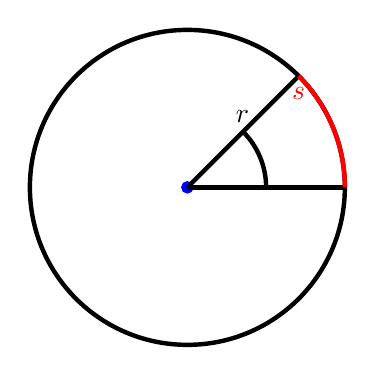
\begin{tikzpicture}
   % \draw[step=1cm,gray,very thin] (3,-3) grid (3,3);
   \filldraw[color = blue, ultra thick](0,0) circle (0.05);
    \draw[ ultra thick](0,0) circle (2);
    \draw[ultra thick] (0,0) -- (1.414,1.414);
  \node[anchor =south] at (0.7,0.7) {$r$};
    \draw[ultra thick] (0,0) -- (2,0);
    \draw[ultra thick] (1,0) arc (0:45:1) node[anchor=north]{$\ut$};
     \draw[ultra thick, color=red] (2,0) arc (0:45:2) node[anchor=north]{$s$};
    \end{tikzpicture}
  %  }{A circle}
    \caption{A circle of radius $r$ showing how arc length around the circle corresponds to angles}
        \label{fig: radians}
\end{figure}

More generally the conversion rule is that
\begin{equation*}
\text{radians} = \frac{180^{\circ}}{\uppi}\times \text{degrees}.
\end{equation*}
The main advantage of radians comes when differentiating and expanding functions as working in degrees requires extra terms to be included and greater care to be taken. While we will not be doing any differentiation in this module we will come across some expressions where we need to work in radians for the quoted expressions to be valid. When this happens we will include a warning so that it is clear where you need to be careful.\\

One way to motivate working in radians is to think of unwinding the circle to get a straight line, for a circle of radius $r$ this length will be the circumference, if we divide this length by $r$ we will have a line if length $2\uppi$ and the angle in radians will be the distance travelled along this line. In other words, working in radians is a bit like converting from circular motion to linear motion.

\begin{figure}[ht]
    \centering
  %  \pdftooltip{
    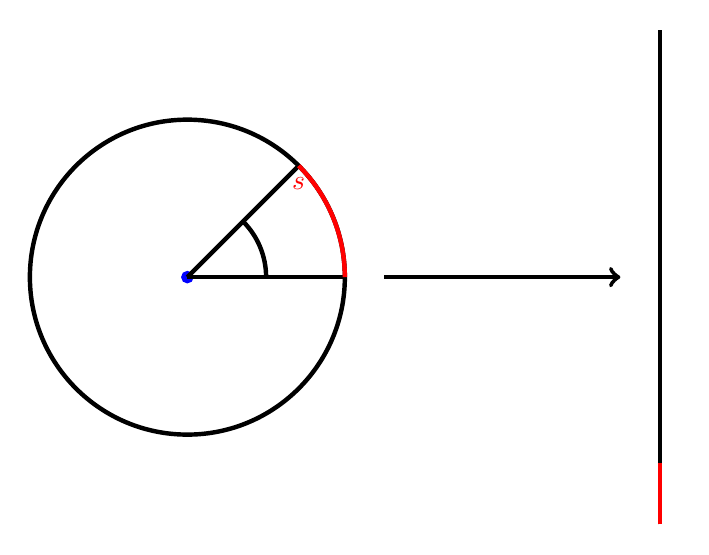
\begin{tikzpicture}
   % \draw[step=1cm,gray,very thin] (3,-3) grid (3,3);
   \filldraw[color = blue, ultra thick](0,0) circle (0.05);
    \draw[ ultra thick](0,0) circle (2);
    \draw[ultra thick] (0,0) -- (1.414,1.414);
 % \node[anchor =south] at (0.7,0.7) {$r$};
    \draw[ultra thick] (0,0) -- (2,0);
    \draw[ultra thick] (1,0) arc (0:45:1) node[anchor=north]{$\ut$};
     \draw[ultra thick, color=red] (2,0) arc (0:45:2) node[anchor=north]{$s$};
     \draw[ultra thick] (6,-3.14) --(6,3.14);
     \draw[ultra thick, color = red] (6,-3.14) --(6,-2.355) node[anchor=west]{$\ut$};
     \draw[ultra thick, ->] (2.5,0) -- (5.5,0);
    \end{tikzpicture}
  %  }{A circle}
    \caption{A circle of radius $r$ showing how arc length around the circle corresponds to angles}
        \label{fig: radians 2}
\end{figure}

As evidenced in \cref{fig: radians,fig: radians 2}, it is common practice to use the Greek letter theta, $\ut$, to denote an angle. Other Greek letters like phi, $\upphi$ or $\upvarphi$, and psi, $\uppsi$, are sometimes used as well. It is worth spending some time familiarising yourself with these Greek letters so you do not think that they are just badly written English letters.

\section{Rearranging Equations}
\label{sec: rearranging}
A very important skill for solving mathematics problems, and finding the roots of functions, is to be able to rearrange equations. This is sometimes referred to as changing the subject of an equation. Newcastle University have a webpage, available \href{https://www.mas.ncl.ac.uk/ask/numeracy-maths-statistics/core-mathematics/pure-maths/algebra/rearranging-equations.html}{here} that goes through some examples of how to rearrange equations. The webpage also has some self test questions that you can look at if you want more practice. Some of the details are reviewed here, along with examples for the specific equations that we have been using in this module.\\


In the equation
\begin{equation*}
x=5y+4z,
\end{equation*}
$x$ is called the subject, which is just a fancy way of saying that $x$ is expressed in terms of the other variables. When we talk about rearranging an equation, we mean that we change the subject of the equation from $x$ to another variable like $y$ and $z$. We do this by performing a variety of mathematical operations to both sides of the equation to swap some of the variables from one side to the other. \\

These operations can include: adding or subtracting a quantity from both sides, multiplying or dividing by a quantity, taking logarithms of or exponentiating both sides of the equation, raising both sides of the equation to any non-zero power.\\
\begin{ex}
Returning to the above equation $x=5y+4x$, we can rearrange it to make $z$ the subject. Again, this means that we will perform mathematical operations on both sides of the equation to put it in the form $z=\dots{}$ : 
\begin{align*}
x&=5y+4z, \quad \text{ first subtract $5y$ from both sides},\\
x-5y&=5y+4z-5y=4z, \quad \text{then divide both sides by 4},\\
\frac{x-5y}{4}&=\frac{4z}{4}=z.
\end{align*}
This gives us
\begin{equation*}
z=\frac{x-5y}{4},
\end{equation*}
with $z$ now the subject of the equation.
\end{ex}

\begin{ex}
As another example consider an equation from physics $v=u+at$, which says that the if an object starts off with a velocity $v$ and accelerates at a rate $a$ then after time $t$ its velocity will be $v$. Here we go through this step by step what we do when solving for $a$:
\begin{align*}
v&=u+at, \quad \text{subtract $u$ from both sides},\\
v-u&=u+at -u=at, \quad \text{divide both sides by $t$},\\
\frac{v-u}{t}&=\frac{at}{t}=a,
\end{align*}
which gives us
\begin{equation*}
a=\frac{v-u}{t}.
\end{equation*}
\end{ex}

\begin{ex}
Another example is rearranging a different equation from physics,
\begin{equation*}
s=ut+\frac{1}{2}at^{2},
\end{equation*}
to solve for either $a$ or $t$.\\

To make $a$ the subject we proceed as follows:
\begin{align*}
s&=ut+\frac{1}{2}at^{2}, \quad \text{subtract $ut$ from both sides},\\
s-ut&=ut+\frac{1}{2}at^{2}-ut=\frac{1}{2}at^{2}, \quad \text{multiply both sides by $2$},\\
2\left(s-ut\right)&=2\left(\frac{1}{2}at^{2}\right)=at^{2}, \quad \text{divide both sides by $t^{2}$},\\
\frac{2\left(s-ut\right)}{t^{2}}&=\frac{at^{2}}{t^{2}}=a,
\end{align*}
thus the equation with $a$ being the subject is 
\begin{equation*}
a=\frac{2\left(s-ut\right)}{t^{2}}.
\end{equation*}

If instead we wanted $t$ to be the subject then it is easier to put it in the form of a quadratic equation and then use the quadratic formula:
\begin{align*}
s&=ut+\frac{1}{2}at^{2}, \quad \text{subtract $s$ from both sides},\\
0&=\frac{1}{2}at^{2}+ut-s,\quad \text{this is a qudratic equation for $t$ and is solved by}\\
t&=\frac{-u\pm\sqrt{u^{2}+2as}}{a}.
\end{align*}
\end{ex}

There are a few special cases where we do not need to use the quadratic formula that it is worth being aware of. If $s=0$ then we have
\begin{align*}
0&=ut+\frac{1}{2}at^{2}, \quad \text{factor out the common factor},\\
0&=t\left(u+\frac{1}{2}at\right),
\end{align*}
This has two solutions $t=0$, which is the start of the motion, and
\begin{align*}
0&=u+\frac{1}{2}at, \quad \text{subtract $u$ from both sides},\\
-u&=\frac{1}{2}at, \quad \text{multiply both sides by $2$},\\
-2u&=at, \quad \text{divide both sides by $a$},\\
-\frac{2u}{a}&=t.
\end{align*}
This case often appear when considering projectile motion and you want to calculate the total length of time that the projectile is in the air for.\\

The other common example is if $u=0$, then:
\begin{align*}
s&=\frac{1}{2}at^{2}, \quad \text{multiply both sides by $2$},\\
2s&=at^{2}, \quad \text{divide both sides by $a$},\\
\frac{2s}{a}&=t^{2}, \quad \text{take the square root of both sides},\\
\sqrt{\frac{2s}{a}}&=t.
\end{align*}
In the last line we have dropped the $\pm$ that should be in front of the square root since we do not consider negative time. However, if you were just solving a quadratic equation then you would have to remember to include that.  Both of these special cases can also be found by direct substitution into the quadratic formula of $s=0$ or $u=0$ respectively.\\

\begin{ex}
The final example is to rearrange an equation involving a square root,
\begin{equation*}
T=2\uppi\sqrt{\frac{l}{g}}.
\end{equation*}
If you are asked to make $l$ the subject of this equation we proceed as follows:
\begin{align*}
T&=2\uppi\sqrt{\frac{l}{g}}, \quad \text{first divide both sides by $2\uppi$},\\
\frac{T}{2\uppi}&=\frac{2\uppi}{2\uppi}\sqrt{\frac{l}{g}}=\sqrt{\frac{l}{g}}, \quad \text{then square both sides of the equation},\\
\left(\frac{T}{2\uppi}\right)^{2}&=\left(\sqrt{\frac{l}{g}}\right)^{2}=\frac{l}{g}, \quad \text{now multiply both sides by $g$},\\
g\left(\frac{T}{2\uppi}\right)^{2}&=g\times\frac{l}{g}=l.
\end{align*}
This leaves us with
\begin{equation*}
l=g\left(\frac{T}{2\uppi}\right)^{2}=\frac{gT^{2}}{4\uppi^{2}}.
\end{equation*}
This is the equation for a straight line $y=mx+c$ where $l$ plays the role of $y$, the $y$-intercept $c=0$, $\left(\frac{T}{2\uppi}\right)^{2}$ plays the role of $x$, and $m=g$ is the gradient of the straight line. When analysing your data you would use plot your data and should observe a straight line whose gradient is $g$.\\

At the last step of this rearrangement we could instead make $g$ the subject. To do this we proceed as follows:
\begin{align*}
\left(\frac{T}{2\uppi}\right)^{2}&=\left(\sqrt{\frac{l}{g}}\right)^{2}=\frac{l}{g}, \quad \text{now multiply both sides by $g$},\\
g\left(\frac{T}{2\uppi}\right)^{2}&=g\times \frac{l}{g}=l, \quad \text{divide both sides by }\left(\frac{T}{2\uppi}\right)^{2}, \\
g&=\frac{l}{\left(\frac{T}{2\uppi}\right)^{2}}=\frac{4\uppi^{2} l}{T^{2}}.
\end{align*}
\end{ex}

If you want more examples there is a \textbf{Transposition of Formulae} workbook, designed by mathcentre,  available \href{https://www.mathcentre.ac.uk/resources/uploaded/mc-ty-transposition-2009-1.pdf}{here}.
